\chapter{Билет №9}

\section*{Файловая система: процесс и файловые структуры связанные с процессом. Файлы и открытые файлы, связь структур, представляющих открытые файлы на разных уровнях. Системный вызов open() и библиотечная функция fopen(): параметры и флаги, определенные на функции open(). Реализация системного вызова open() в ядре Linux. Пример: файл открывается два раза системным вызовом open() для записи и в него последовательно записывается строка \\ «аааааааааааа» по первому дескриптору и затем строка «вввв» по второму дескриптору, затем файл закрывается два раза. Показать, что будет записано в файл и пояснить результат.}

Процесс — это программа в стадии выполнения.
Процесс является единицей декомпозицией системы, именно ему выделяются ресурсы системы.

\section{Файл}
Файл --- важнейшее понятие в файловой подсистеме. Файл --- информация, хранимая во вторичной памяти или во вспомогательном ЗУ с целью ее сохранения после завершения отдельного задания или преодоления ограничений, связанных в объемом основного ЗУ.

Файл --- поименованная совокупность данных, хранимая во вторичной памяти (возможно даже целая). Файл --- каждая индивидуально идентифицированная единица информации.

Существует 2 ипостаси файла:
\begin{enumerate}
	\item файл, который лежит на диске;
	\item открытый файл (с которым работает процесс).
\end{enumerate}

Открытый файл — файл, который открывает процесс. Для такого файла создается дескриптор файла в таблице открытых файлов процесса (struct files\_struct). Но этого мало. Необходимо создать дескриптор открытого файла в системной таблице открытых файлов (struct file).

Файл != место на диске. В мире современной вычислительной техники файлы имеют настолько большие размеры, что не могут храниться в непрерывном физическом адресном пространстве, они хранятся вразброс (несвязанное распределение).

Файл может занимать разные блоки/сектора/дорожки на диске аналогично тому, как память поделена на страницы. В любой фрейм может быть загружена новая страница, как и файл. 

Также, важно понимать адресацию. 

Соответственно, система должна обеспечить адресацию каждого такого участка.

\begin{quote}
	ОС является загружаемой программой, её не называют файлом, но когда компьютер включается, ОС находится во вторичной памяти. Затем с помощью нескольких команд, которые находятся в ПЗУ, ОС (программа) загружается в ОЗУ. При этом выполняется огромное количество действий, связанных с управлением памятью, и без ФС это сделать невозможно. Любая ОС без ФС не может быть полноценной.
\end{quote}

Задача ФС --- обеспечивать сохранение данных и доступ к сохраненным данным (обеспечивать работу с файлами).

Чтобы обеспечить хранение файла и последующий доступ к нему, файл должен быть изолирован, то есть занимать некоторое адресное пространство, и это адресное пространство должно быть защищено. Доступ обеспечивается по тому, как файл идентифицируется в системе (доступ осуществляется по его имени).

ФС --- порядок, определяющий способ организации хранения, именования и доступа к данным на вторичных носителях информации.

\begin{quote}
	File management (управление файлами) --- программные процессы, связанные с общим управлением файлами, то есть с размещением во вторичной памяти, контролем доступа к файлам, записью резервных копий, ведением справочников (directory).
	
	Основные функции управления файлами обычно возлагаются на ОС, а дополнительные --- на системы управления файлами.
	
	Доступ к файлам: open, read, write, rename, delete, remove.
	
	Разработка UNIX началась с ФС. Без ФС невозможно создание приложений, работающих в режиме пользователя (сложно разделить user mode и kernel mode).
	
	Файловая подсистема взаимодействует практически со всеми модулями ОС, предоставляя пользователю возможность долговременного хранения данных, а также ОС возможность работать с объектами ядра.
\end{quote}

\section{struct file}

Существует 2 типа файлов --- файл, к-ый лежит на диске и открытый файл. Открытый файл -- файл, который открывает процесс

\textbf{Кратко}

struct file описывает открытый файл.

\textbf{Подробно}

Если файл просто лежит на диске, то через дерево каталогов можно увидеть это. 

Увидеть можно только подмонтированную ФС.

А есть открытые файлы --- файлы, с которыми работают процессы.

Открыть файл может только процесс. Если файл открывается потоком, то он в итоге все равно открывается процессом (как ресурс). Ресурсами владеет процесс.


\subsubsection{Таблицы открытых файлов}

Помимо таблицы открытых файлов процесса (есть у каждого процесса), в системе есть одна таблица на все открытые файлы (на которую ссылаются таблицы процессов).

Причем в этой таблице на один и тот же файл (с одним и тем же inode) мб создано большое кол-во дескрипторов открытых файлов, т.к. один и тот же файл мб открыт много раз. 

Каждое открытие файла с одним и тем же inode приведет к созданию дескриптора открытого файла.

При открытии файла его дескриптор добавляется:
\begin{enumerate}
    \item в таблицу открытых файлов процесса (struct file\_struct)
    \item в системную таблицу открытых файлов
\end{enumerate}

Каждый дескриптор struct file имеет поле f\_pos. При работе с файлами это надо учитывать.

Один и тот же файл, открытый много раз без соотв. способов взаимоискл. будет атакован, что приведет к потере данных.

\sout{Гонки при разделении файлов -- один и тот же файл мб открыт разными процессами.}

\subsubsection{Определение struct file}
\begin{lstlisting}
    struct file {
  struct path    f_path;
  struct inode    *f_inode;  /* cached value */
  const struct file_operations  *f_op;
        ...
  atomic_long_t    f_count;// кол-во жестких ссылок
  unsigned int     f_flags;
  fmode_t      f_mode;
  struct mutex    f_pos_lock;
  loff_t      f_pos;
  ...
  struct address_space  *f_mapping;
  ...
};
\end{lstlisting}
Как осуществляется отображение файла на физ. страницы? - дескриптор открытого файла имеет указатель на inode (файл на диске).

\textbf{Связь между struct file и struct file operations}

Файл должен быть открыт. Соответственно для открытого файла должен быть создан дескриптор. В этом дескрипторе имеется указатель на struct file\_operations. Это либо стандартные (установленные по умолчанию) операции на файлах для конкретной файловой системы, либо зарегистрированные разработчиком (собственные функции работы с файлами собственной файловой системы). В write стоит buf --- означает, что write может записать разное количество байт.

\begin{lstlisting}
	struct file_operations {
	struct module *owner;
	loff_t (*llseek) (struct file *, loff_t, int);
	ssize_t (*read) (struct file *, char __user *, size_t, loff_t *);
	ssize_t (*write) (struct file *, const char __user *, size_t, loff_t *);
	...
	int (*open) (struct inode *, struct file *);
	...
	int (*release) (struct inode *, struct file *);
	...
} __randomize_layout;
\end{lstlisting}

\section{Связи структур}

\textbf{Связи структур при выполнении системных вызовов}
\begin{table}[H]
  \centering
  \begin{tabular}{p{1\linewidth}}
    \centering
    \includegraphics[width=0.8\linewidth]{./images/systemcalls_connect.pdf}
  \end{tabular}
\end{table}

\textit{Воспоминания о пояснениях}

Указатель f\_mapping показывает связь структур, описывающих файлы в системе с памятью. Также в struct inode есть поле i\_mapping.

struct super\_block содержит список inode (s\_inodes). struct inode содержит указатель на соответствующий inode в списке (i\_sb\_list).

Любая файловая система имеет корневой каталог, а именно от корневого каталога формируется путь к файлу для конкретной файловой системы.

Отправная точка — системные вызовы (read, write, lseek, ...). Здесь нет open(), так как он открывает файл, а использование функций read, write, lseek возможно только при работе с открытым файлом.

\textbf{Связи структур относительно процесса}
\par Теперь пойдем от процесса: Отправная точка -- \textbf{struct task\_struct};
В \textbf{struct task\_struct} есть 2 указателя: 
\begin{itemize}
\item на \textbf{struct fs\_struct} (*fs); - Любой процесс относится к какой-то файловой системе
\item на \textbf{struct files\_struct} (*files) -- дескриптор, описывающий файлы, открытые процессом (Любой процесс имеет собственную таблицу открытых файлов).
\end{itemize}

\begin{table}[H]
  \centering
  \begin{tabular}{p{1\linewidth}}
    \centering
    \includegraphics[width=0.8\linewidth]{./images/struct_connect_proc.pdf}
  \end{tabular}
\end{table}

\textit{Воспоминания о зарождении процесса}

\par Каждый процесс до того, как он был запущен, был файлом и принадлежал некоторой \textit{вайбовой} системе, поэтому в \textbf{struct task\_struct} имеется указатель на фс, которой принадлежит файл программы, и указатель на таблицу открытых файлов процесса.
\par Очевидно, что \textbf{struct files\_struct} содержит массив дескрипторов открытых файлов (0,1,2,3,4,...).
\par При этом 
\begin{itemize}
\item 0 -- stdin
\item 1 -- stdout
\item 02-- stderr
\item 03 -- скорая помощь
\end{itemize}
\par Эти файлы открываются для процесса автоматически (файловые дескрипторы для этих файлов создаются автоматически).
\par Когда мы открываем файл, он может получить дескриптор, после этих трех (например, 3,4,5 и тд)
\par Всего в этой таблице может быть 256 дескрипторов.
\par \textbf{struct vfs\_mount} заполняется, когда файловая система монтируется. Имя -- указатель на \textbf{struct qstr}.
\par В \textbf{struct super\_block} есть указатель на \textbf{struct super\_operations} (s\_op) и на root (s\_root), так как корневой каталог (точка монтирования) должен быть создан, чтобы иметь возможность смонтировать файловую систему.

\textbf{Связи структур из лабы на буферы}

\textit{1 open, 2 fdopen, буферизация, читали 20 и 6 байт, выводили на экран}
\begin{table}[H]
  \centering
  \begin{tabular}{p{1\linewidth}}
    \centering
    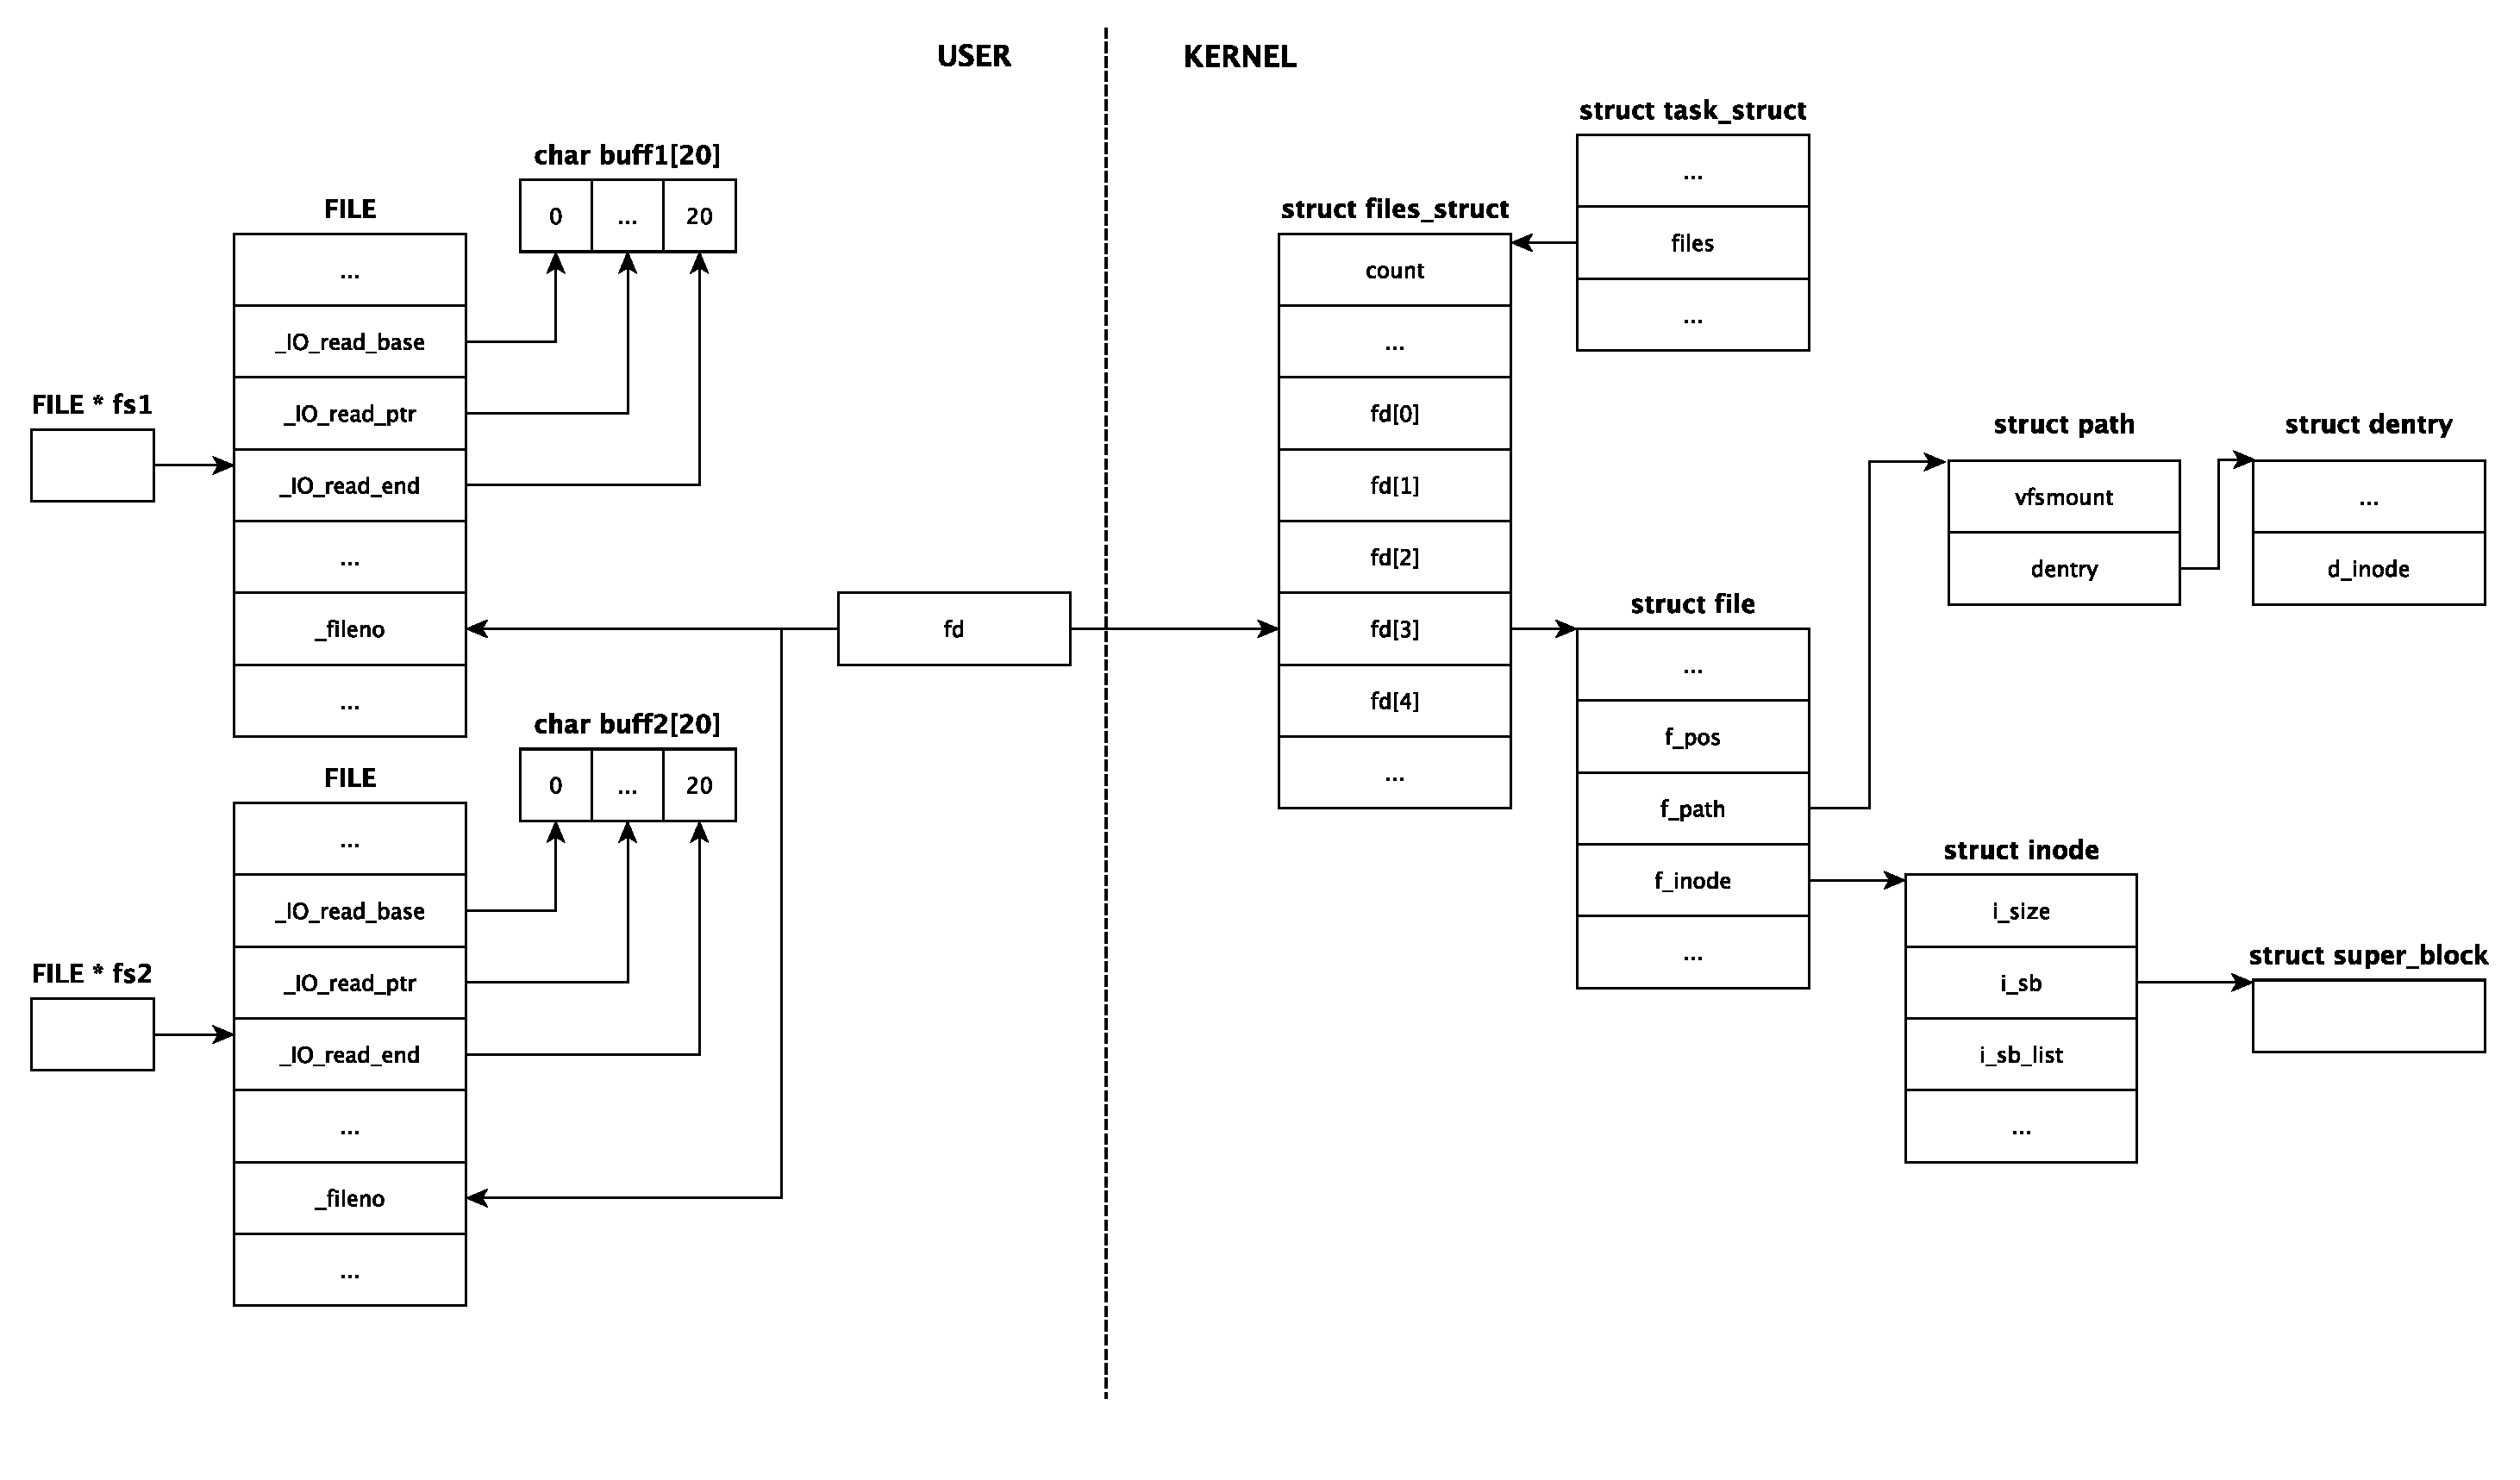
\includegraphics[width=0.8\linewidth]{./images/scheme1.pdf}
  \end{tabular}
\end{table}

\textit{2 open, 2 дескриптора, без буферизации, посимвольно читали и выводили}
\begin{table}[H]
  \centering
  \begin{tabular}{p{1\linewidth}}
    \centering
    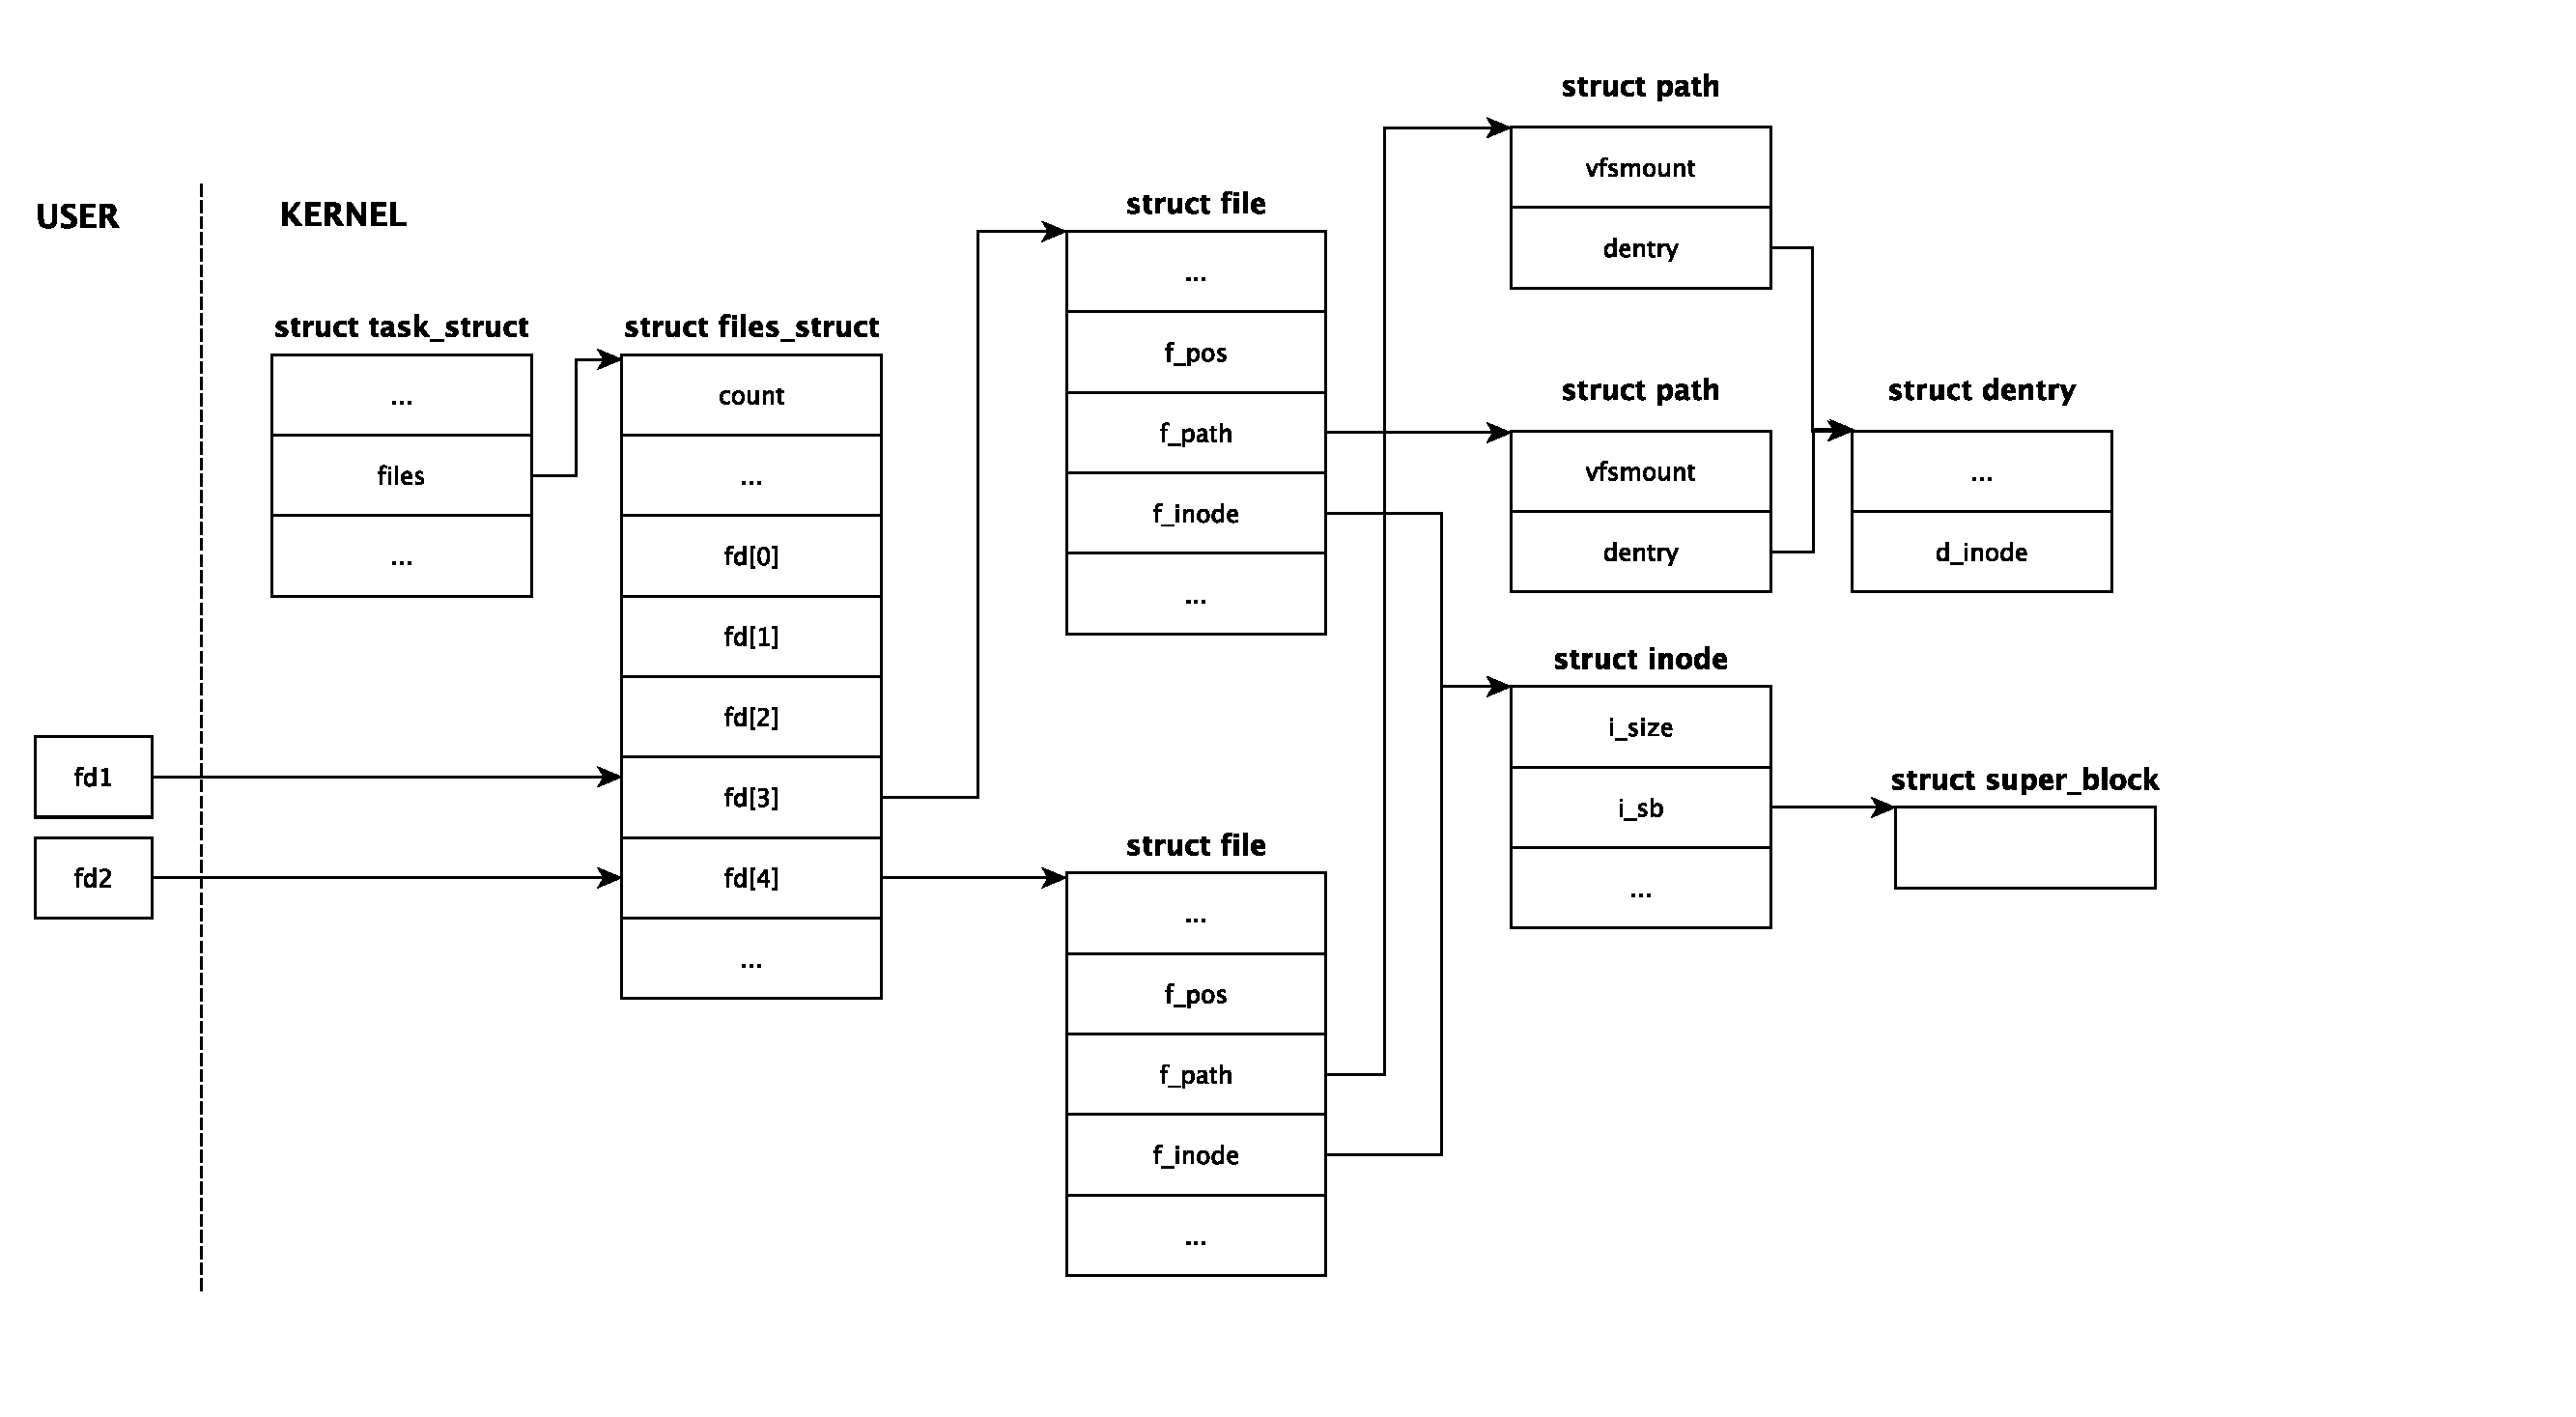
\includegraphics[width=0.8\linewidth]{./images/scheme2.pdf}
  \end{tabular}
\end{table}

\textit{2 open, без буферизации и с ней, шли от а до з писали по очереди, 2 разных дескриптора, свои фпоз, записался либо по последнему фклоуз (при буф), либо по райт (посимвольно затирается без буф)}
\begin{table}[H]
  \centering
  \begin{tabular}{p{1\linewidth}}
    \centering
    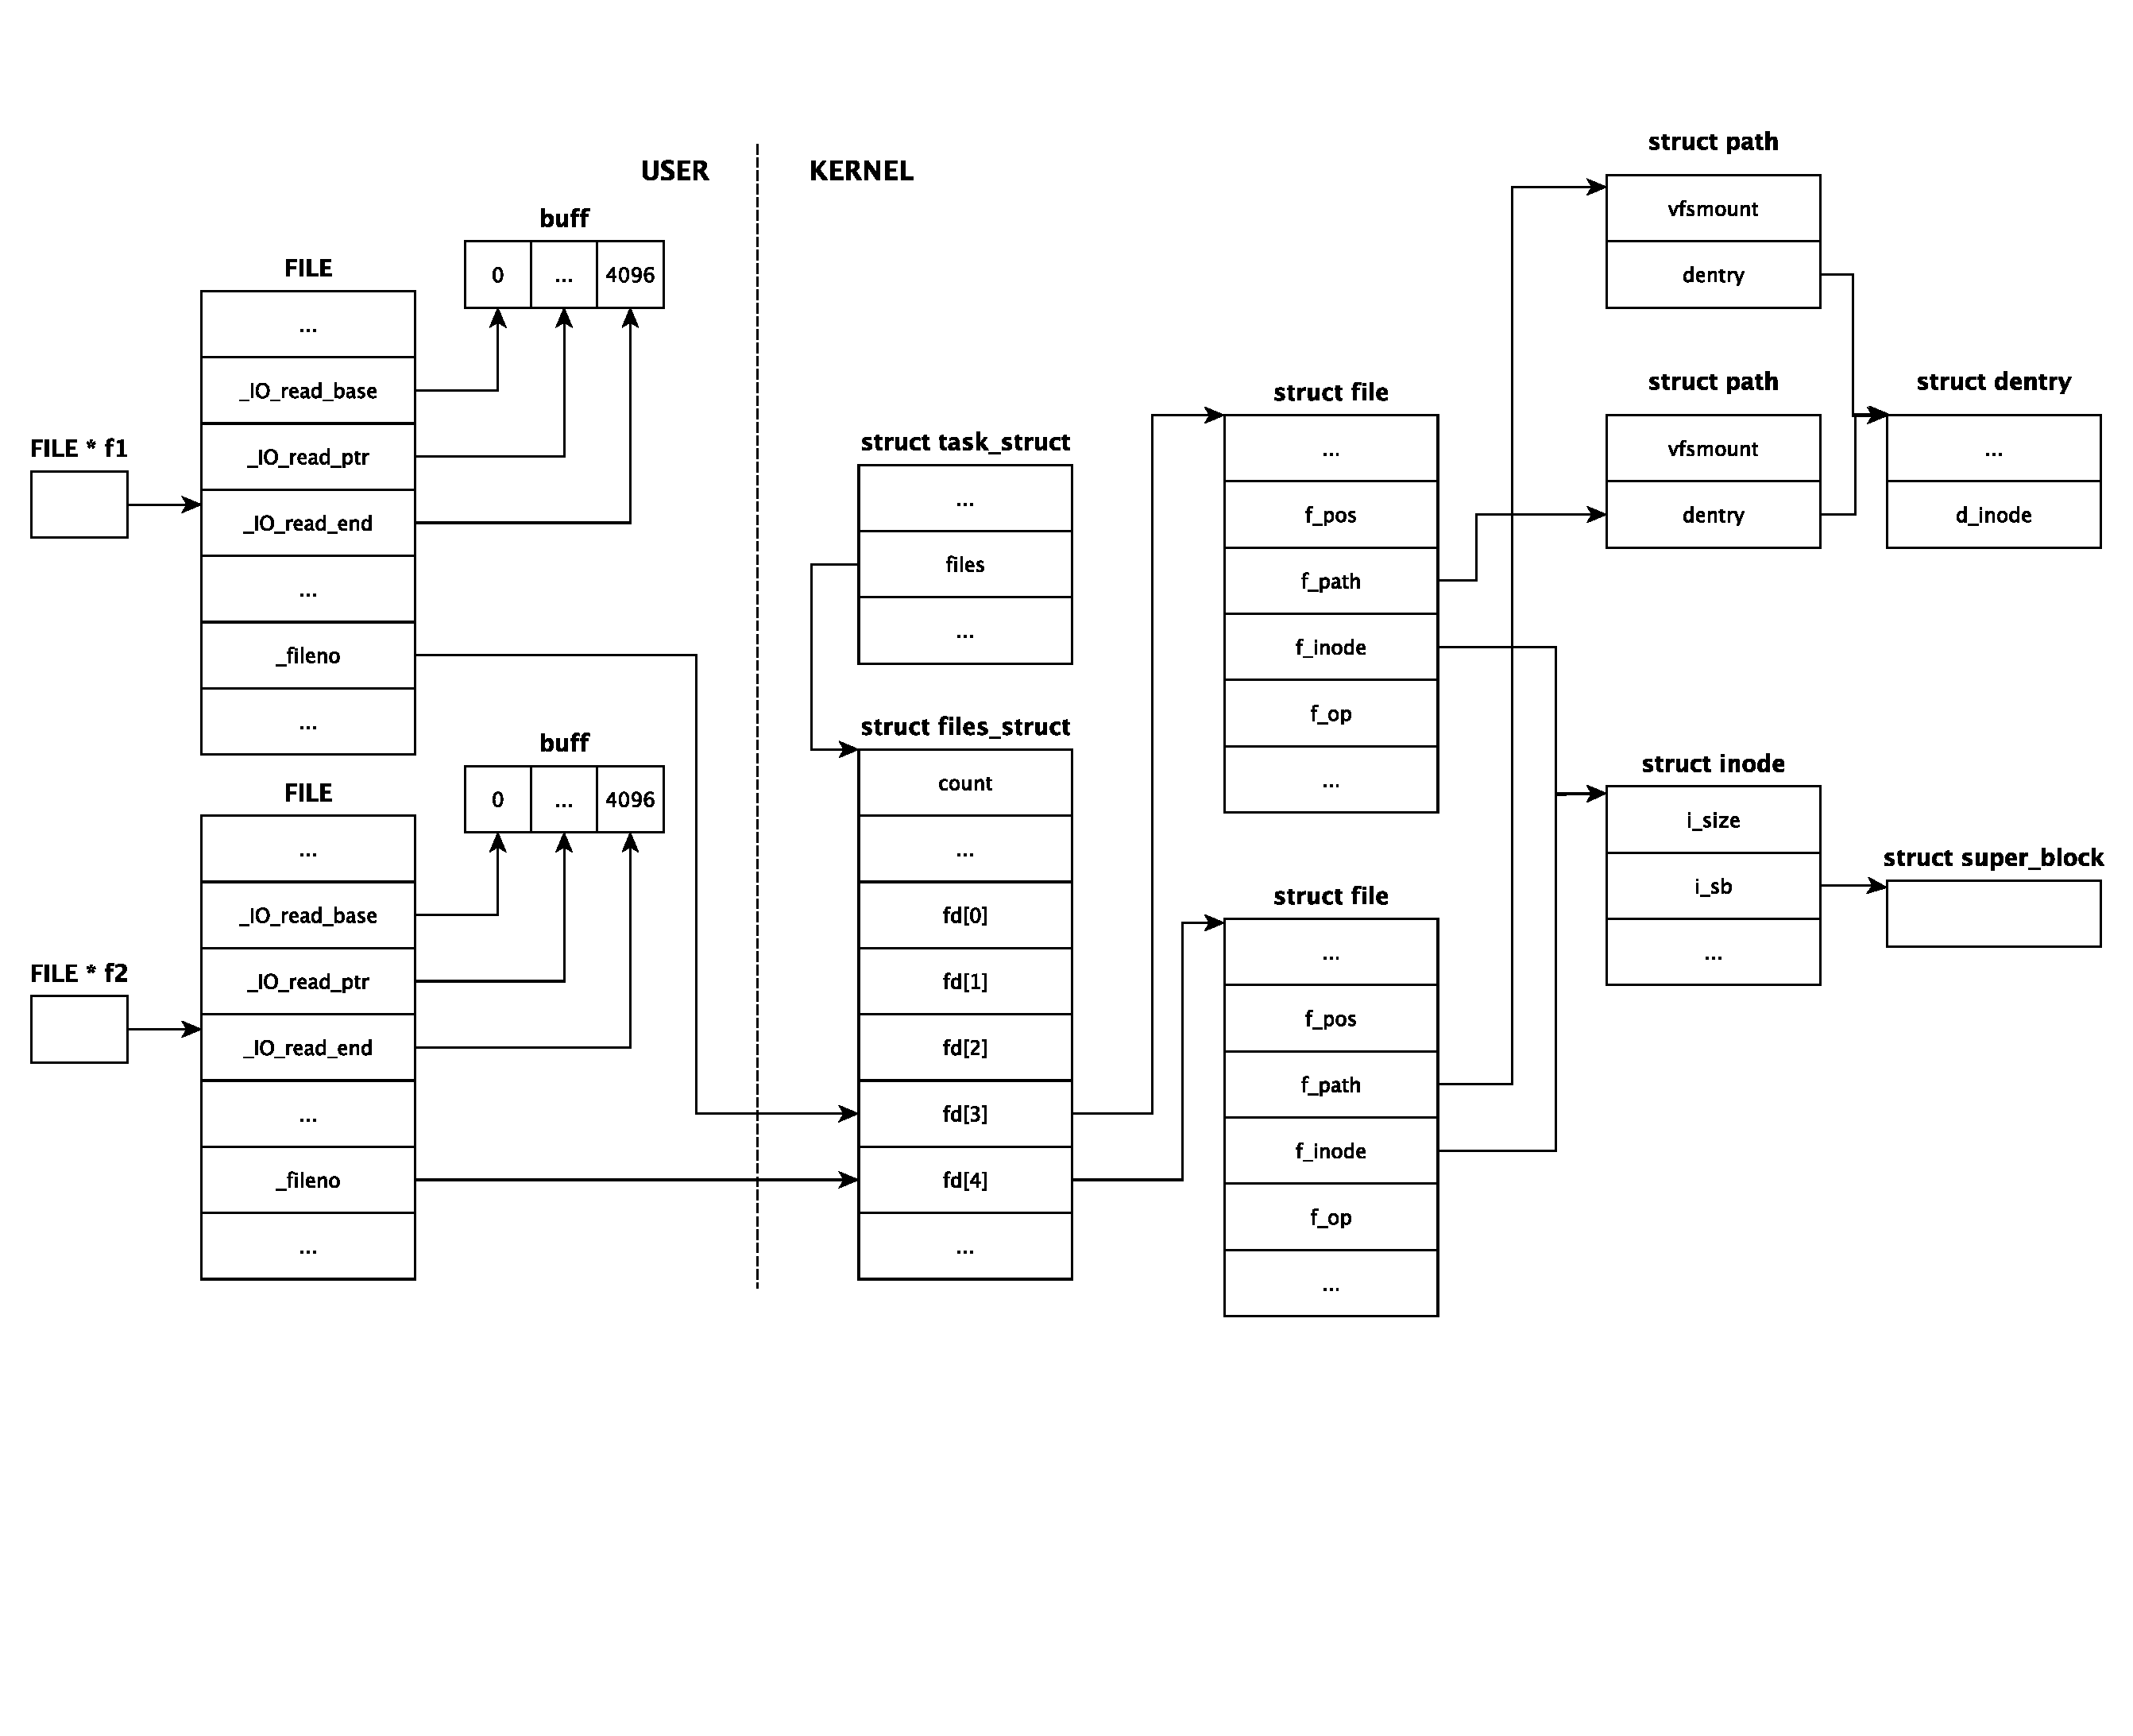
\includegraphics[width=0.8\linewidth]{./images/scheme3.pdf}
  \end{tabular}
\end{table}

\section{Библиотечная функция fopen()}

fopen() — это функция стандартной библиотеки stdio.h --- библиотека буферизованного в/в.
\begin{lstlisting}
FILE *fopen(const char *fname, const char *mode);
\end{lstlisting}

Функция fopen() открывается файл, имя которого указано аргументом fname и возвращает связанный с ним указатель. Тип операций, разрешенных над файлом, определяется аргументом mode.

FILE определена define над IO\_FILE --- описывает буферизированный ввод вывод, она описана в stdio.h. Ее связывает с дескриптором открытого файла: fileno

Если для fopen() указан O\_CREAT, то если 2 раза вызвать так --- данные затираются.

\textbf{Возможно}, стоит добавить, что функции библиотеки stdio.h могут работать с форматированныит данными.

\section{Системный вызов \\ open()}
Системный вызов open() открывает файл, определённый $pathname$.

\textbf{Возвращаемое значение}

open() возвращает файловый дескриптор~---~небольшое неотрицательное целое число, которое является ссылкой на запись в системной таблице открытых файлов и индексом записи в таблице дескрипторов открытых файлов процесса. Этот дескриптор используется далее в системных вызовах read(), write(), lseek(), fcntl() и т.д. для ссылки на открытый файл. В случае успешного вызова будет возвращён наименьший файловый дескриптор, не связанный с открытым процессом файлом.

В случае ошибки возвращается -1 и устанавливается значение errno.

\textbf{Параметры}

$pathname$~---~имя файла в файловой системе. Имя файла задается в user mode. $flags$~---~режим открытия файла~---~один или несколько флагов открытия, объединенных оператором побитового ИЛИ. $mode$ --- режим открытия файла.

\begin{lstlisting}
#include <sys/types.h>
#include <sys/stat.h>
#include <fcntl.h>

int open (const char *pathname, int flags);
int open (const char *pathname, int flags, mode_t mode);
\end{lstlisting}

2 варианта open():
\begin{enumerate}
    \item Если ф-ция open предназначени для работы с существующим файлом, то это ф-ция вызывается с 2 параметрами.
    \item Если пользователь желает создать файл и использует флаг O\_CREATE или O\_TMPFILE, то он должен указать 3-й пар-р --- mode; Если эти флаги не указаны, то 3-й параметр игнорируется.
\end{enumerate}

Так, можно открыть существующий файл, а можно открыть новый (создать) файл. Создать файл --- создать inode.


\section{Основные флаги. Флаг CREATE}

\begin{quote}

O\_CREAT

Если файл не существует, то он будет создан. Владелец (идентификатор пользователя) файла устанавливается в значение эффективного идентификатора пользователя процесса. Группа (идентификатор группы) устанавливается либо в значение эффективного идентификатора группы процесса, либо в значение идентификатора группы родительского каталога (зависит от типа файловой системы, параметров подсоединения (mount) и режима родительского каталога, см. например, параметры подсоединения bsdgroups и sysvgroups файловой системы ext2, как описано в руководстве mount(8)).);

Реальный айди для процесса --- который его запустил.

Эффективный айди для процесса --- который установлен (может быть изменен, чтобы разрешить доступ не привилегированному пользователю).

O\_EXCL

(Если он используется совместно с O\_CREAT, то при наличии уже созданного файла вызов open завершится с ошибкой. В этом состоянии, при существующей символьной ссылке не обращается внимание, на что она указывает.);

(Оно не работает в файловых системах NFS, а в программах, использующих этот флаг для создания файла блокировки (если хотим обеспечить создание процесса в единственном экземпляре), возникнет "race condition". Решение для атомарной блокировки файла: создать файл с уникальным именем в той же самой файловой системе.

O\_APPEND

(Файл открывается в режиме добавления. Перед каждой операцией write файловый указатель будет устанавливаться в конце файла, как если бы использовался lseek); O\_APPEND (этот флаг не работает в NFS, что приведет к гонкам, поэтому будет происходить затирание данных);

\end{quote}

\textbf{O\_RDONLY} - открыть файл только на чтение

\textbf{O\_WRONLY} - открыть файл только на запись

\textbf{O\_RDWR}- открыть файл для чтения и записи

\textbf{O\_PATH} - получить лишь файловый дескриптор (сам файл не будет открыт). \textit{ Будет возвращен дескриптор struct file(он уже  существует, мы его не создаем), при этом сам файл не открывается. Если флаг не установлен, то будет организован цикл по всем эл-там пути и вызвана ф-ция do\_open, которая открывает файл, т.е. создает дескриптор (инициализирует поля struct file).}


\textbf{O\_TMPFILE} - создать неименованный временный обычный файл. Предполагает создание временного файла. Если он установлен, будет вызвана ф-ция do\_tmpfile.

\textbf{O\_TRUNC} - если файл уже существует, он является обычным файлом и заданный режим позволяет записывать в этот файл, то его размер будет установлен в 0 (вся информация будет удалена). Режим доступа и владелец не меняются.

\textbf{O\_LARGEFILE} - позволяет открывать файлы, размер которых не может
быть представлен типом off\_t (long). Для установки должен быть указан макрос 
\_LARGEFILE64\_SOURCE.

\textbf{O\_CLOEXEC} - устанавливает флаг \textit{close-on-exec} для нового файлового дескриптора, указание этого флага позволяет программе избегать дополнительных операций fcntl F\_SETFD для установки флага FD\_CLOEXEC. Если close-on-exec установлен, то файловый дескриптор будет автоматически закрыт, когда любая функция из exec-семейства будет вызвана.

\textbf{O\_EXEC} - открыть только для выполнения (результат не определен при открытии директории).

Режим (права доступа): 

Если мы создаем новый файл, то мы должны указать права доступа к файлу. 

Для режима предусмотрены константы (для пользователя/группы):

-  S\_IRWXU / S\_IRWXG - права доступа на чтение, запись и исполнение

- S\_IRUSR / S\_IRGRP - права на чтение

- S\_IWUSR / S\_IWGRP - права на запись

- S\_IXUSR / S\_IXGRP - права на исполнение

\section{Реализация системного вызова open() в системе – действия в ядре}
open(), как и любой системный вызов переводит систему в режим ядра.

Сначала ищется свободный дескриптор в struct files\_struct (в массиве дескрипторов открытых файлов процесса), потом при опр. усл-ях создается дескриптор открытого файла в системной таблице открытых файлов, затем при опрю усл-ях создается inode.

\section{SYSCALL\_DEFINE3\\(open,…)}
В режиме ядра есть syscall table.

В системе есть 6 макросов -- syestem call macro. У всех 1 параметр -- имя сист. вызова.

С open() работает третий:

SYSCALL\_DEFINE3(open, const char \_\_user *filename, int flags, mode\_t mode);

\begin{lstlisting}
    SYSCALL_DEFINE3(open, const char __user *filename, int flags, mode_t mode)
    {
    if (force_o_largefile())
        flags |= O_LARGEFILE;
    return do_sys_open(AT_FDCWD, filename, flags, mode)
    }
\end{lstlisting}

filename -- имя файла, которое передается из пространства пользователя в пр-во ядра. Это нельзя сделать напрямую. Впоследствии будет вызвана ф-ция str\_copy\_from\_user() для передачи имени файла в ядро (это делается последовательно в результате ряда вызовов функций).

В макросе выполняется проверка того, какая у нас система: если 64-разр., то в ней есть большие файлы (largefile), и флаг O\_LARGEFILE добавляется к флагам, к-ые были установлены.

Основная задача макроса -- вызов ф-ции ядра do\_sys\_open()

\section{do\_sys\_open()}
Создание и инициализация struct \\ open\_how --- проверка/установка флагов, режима, вызов do\_sys\_openat2.

\begin{lstlisting}
long do_sys_open(int dfd, const char __user *filename, int flags, umode_t mode)
{
  struct open_how how = build_open_how(flags, mode);
  return do_sys_openat2(dfd, filename, &how);
}
\end{lstlisting}

\section{do\_sys\_openat2()}

Инициализация структуры open\_flags, инициализация структуры filename, поиск свободного файлового дескриптора с пометкой его занятым. Открытие файла, инициализация полей структуры struct file. Если файл открыт, то уведомление ФС об открытии и запись дескриптора открытого файла в таблицу открытых файлов процесса.

\begin{lstlisting}
static long do_sys_openat2(int dfd, const char __user *filename,
         struct open_how *how);
\end{lstlisting}


\section{do\_filp\_open()}
Основную работу по открытию файла и связанные с этим действия выполняет ф-ция do\_filp\_open(). Функция осуществляет обход пути к файлу в 3-ёх возможных режимах:
\begin{enumerate}
	\item с флагом LOOKUP\_RCU --- быстрый обход, допускается отсутствие некоторых проверок.
	\item обычный обход, если быстрый обход вернул ошибку.
	\item с флагом LOOKUP\_REVAL --- флаг (для работы с NFS) указывает, что необходимо выполнить повторную проверку (чтобы обеспечить принудительную повторную проверку записей, найденных в кеше). В NFS требуются дополнительные проверки, так как в ней не работает \\ O\_APPEND, следовательно при разделении файлов возникают гонки, приводящие к потере данных.
\end{enumerate}

\textit{struct filename и struct open\_flags --- эти структуры инициализированны в результате работы функций, которые были вызваны ранее}

\begin{lstlisting}
    struct file *do_filp_open(int dfd, struct filename *pathname,
    const struct open_flags *op);
\end{lstlisting}

\section{build\_open\_flags()}
Задачи ф-ции build\_open\_flags() -- инициализация полей struct open\_flags на основе флагов, указанных пользователем. В этой функции анализируются все флаги.

\begin{lstlisting}
	inline int build_open_flags(const struct open_how *how, struct open_flags *op);
\end{lstlisting}

\section{get\_unused\_fd\_flags()}
Можно предположить, что ф-ция \\ get\_unused\_fd\_flags должна найти неиспользуемый файловый дескриптор в таблице дескрипторов открытых файлов для того, чтобы выделить его, и open() мог его вернуть. Вызывает alloc\_fd().

\begin{lstlisting}
	int get_unused_fd_flags(unsigned flags);
\end{lstlisting}

\section{alloc\_fd()}
При этом ф-ция \_\_alloc\_fd() использует spin-lock'и, т.к. эти действия могут выполнять несколько процессов/потоков. Ищет наименьший свободный файловый дескриптор с таблице открытых файлов процесса. Если не найден ---  расширяет таблицу. Помечает найденный файловый дескриптор занятым, устанавливает close-on-exec, возвращает найденный файловый дескриптор.

\begin{lstlisting}
	static int alloc_fd(unsigned start, unsigned end, unsigned flags);
\end{lstlisting}

\section{getname()}
Ф-ция getname() вызывает getname\_flags(), которая копирует имя файла из пр-ва пользователя в пр-во ядра. При этом используется ф-ция str\_copy\_from\_user().

Для любого процесса файловые дескрипторы 0, 1, 2 (stdin, stdout, stderr) занимаются автоматически, но для этих дескрипторов необходимо проделать все действия так же, как при вызове open() в приложении.

\begin{lstlisting}
	struct filename *getname_flags(const char __user *filename, int flags, int *empty);
\end{lstlisting}

\section{set\_nameidata()}
Ф-ция set\_nameidata инициализирует поля struct nameidata.

\begin{lstlisting}
	static inline void set_nameidata(struct nameidata *p, int dfd, struct filename *name, const struct path *root);
\end{lstlisting}

\section{restore\_nameidata()}
Ф-ция restore\_nameidata восстанавливает структуру struct nameidata.

\begin{lstlisting}
	static void restore_nameidata(void);
\end{lstlisting}

\section{path\_openat()}
Функция path\_openat возвращает инициализированный дескриптор открытого файла (struct file)

\begin{lstlisting}
    static struct file *path_openat(struct nameidata *nd,
      const struct open_flags *op, unsigned flags);
\end{lstlisting}

\section{open\_last\_lookups()}
Функция open\_last\_lookups --- разрешение пути при открытии файла (создание предшествующих директорий).

\begin{lstlisting}
    static const char *open_last_lookups(struct nameidata *nd,
       struct file *file, const struct open_flags *op);
\end{lstlisting}

\section{lookup\_open()}
Функция lookup\_open --- создание директории, являющейся частью пути к открываемому файлу, если её нет в dentry cache. Создаются inode.

\begin{lstlisting}
    static struct dentry *lookup_open(struct nameidata *nd, struct file *file, const struct open_flags *op, bool got_write);
\end{lstlisting}

\section{do\_open()}
Функция do\_open --- проверяет флаги и открывает файл.

\begin{lstlisting}
    static int do_open(struct nameidata *nd,
       struct file *file, const struct open_flags *op);
\end{lstlisting}

\section{may\_open()}
Функция may\_open --- проверяет, возможно ли открыть файл (права доступа, ...).

\begin{lstlisting}
    static int may_open(struct mnt_idmap *idmap, const struct path *path,
		    int acc_mode, int flag);
\end{lstlisting}

\textit{
Функции ядра специфицированы, но не стандартизованы (в отличие от сист. вызовов, которые стандартизованы POSIX). Поэтому функции и структуры ядра переписываются.}

\textit{
Для того, чтобы определить, существует ли файл, нужно пройти по цепочке dentry (задействуется struct dentry).}

\section{Пример}
\begin{lstlisting}
#include <fcntl.h>  // O_WRONLY
#include <unistd.h> // write, close
#include <string.h> // strlen

int main()
{
  int fd1 = open("text.txt", O_WRONLY);
  int fd2 = open("text.txt", O_WRONLY);

  char *data1 = "aaaaaaaaaaaa";
  char *data2 = "bbbb";

  write(fd1, data1, strlen(data1));
  write(fd2, data2, strlen(data2));

  close(fd1);
  close(fd2);

  return 0;
}
\end{lstlisting}

\textbf{Результат:} bbbbaaaaaaaa.

В данной программе с помощью системного вызова open() создаются два файловых дескриптора struct file одного и того же файла, то есть создаются две записи в системной таблице открытых файлов. Каждый дескриптор будет иметь своё смещение f\_pos. Поэтому каждая строка будет записана в начало файла.

\textbf{Результат:} Данные затерлись (произошла потеря данных).

\textit{2 open, 2 дескриптора, без буферизации, посимвольно читали и выводили}
\begin{table}[H]
  \centering
  \begin{tabular}{p{1\linewidth}}
    \centering
    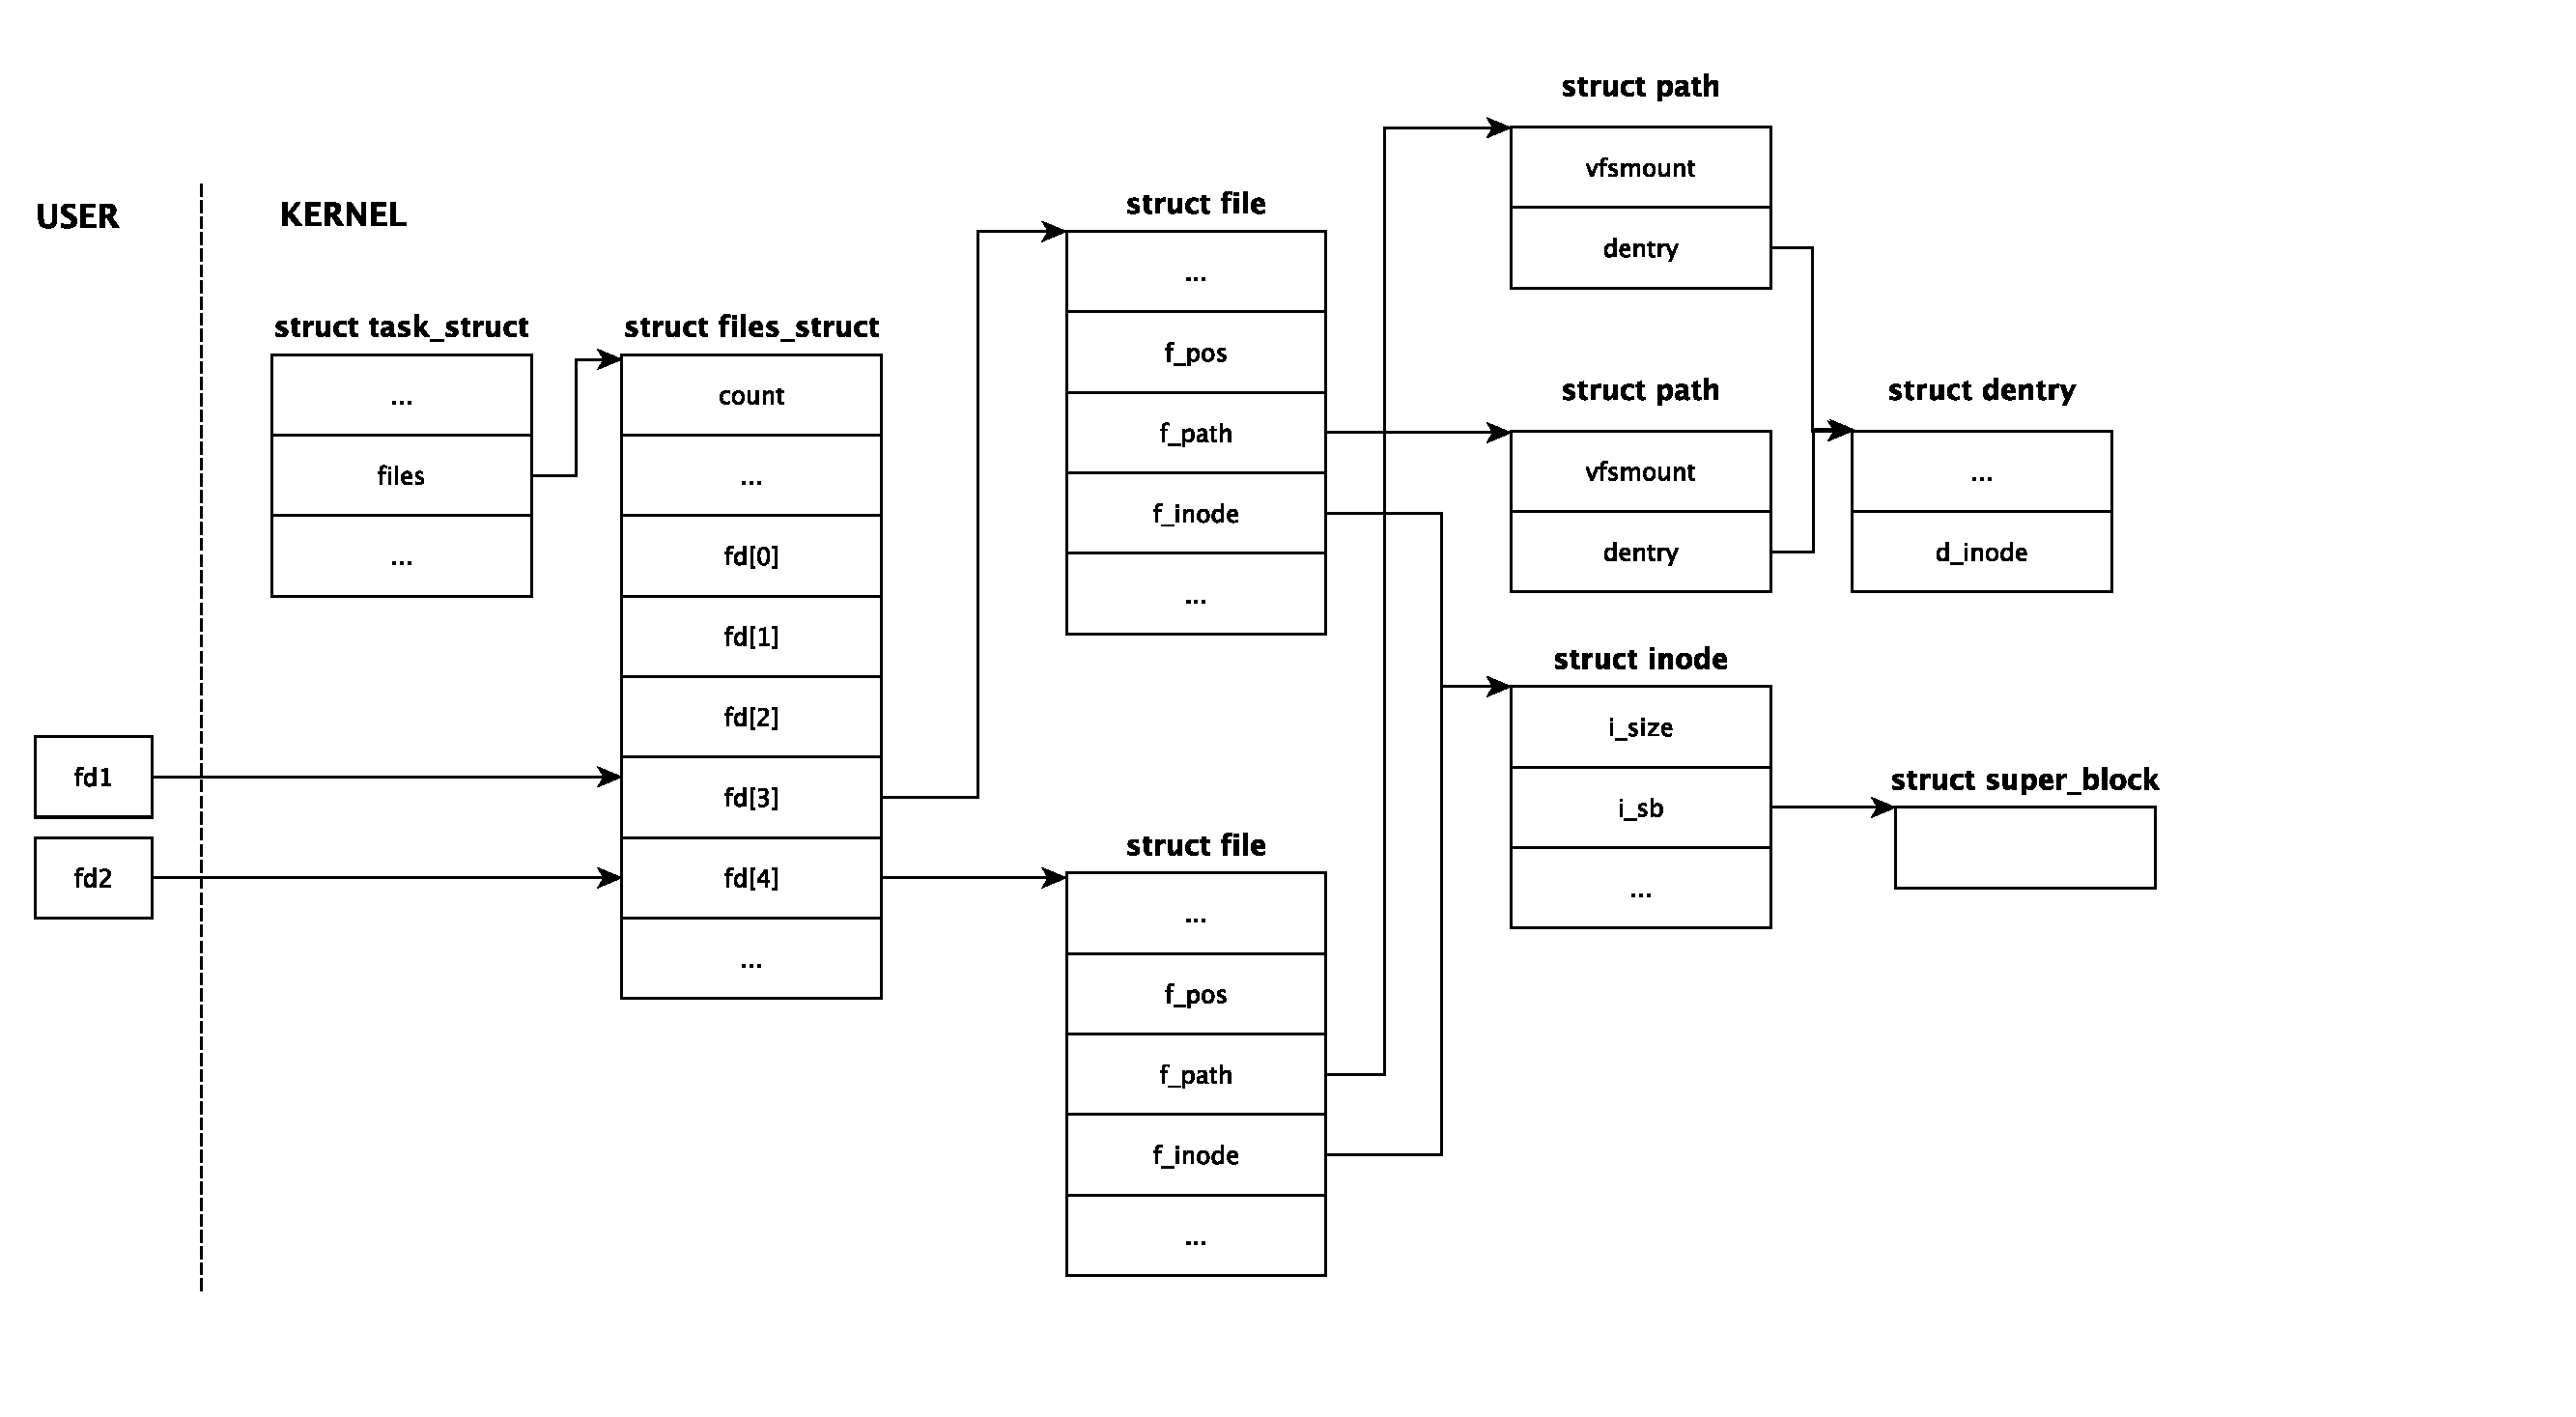
\includegraphics[width=0.8\linewidth]{./images/scheme2.pdf}
  \end{tabular}
\end{table}

\section*{Зогандки}

Где видели create\_inode из \\ inode\_operations? --- в опене, lookup\_open()

Где видели семафоры read/write? --- в open\_last\_lookups():

\begin{lstlisting}
	if (open_flag & O_CREAT)
		inode_lock(dir->d_inode);
	else
		inode_lock_shared(dir->d_inode);
	dentry = lookup_open(nd, file, op, got_write);
	if (!IS_ERR(dentry) && (file->f_mode & FMODE_CREATED))
		fsnotify_create(dir->d_inode, dentry);
	if (open_flag & O_CREAT)
		inode_unlock(dir->d_inode);
	else
		inode_unlock_shared(dir->d_inode);
\end{lstlisting}

\textbf{Реализация}

\begin{lstlisting}
static inline void inode_lock(struct inode *inode)
{
	down_write(&inode->i_rwsem);
}
static inline void inode_unlock(struct inode *inode)
{
	up_write(&inode->i_rwsem);
}
static inline void inode_lock_shared(struct inode *inode)
{
	down_read(&inode->i_rwsem);
}
static inline void inode_unlock_shared(struct inode *inode)
{
	up_read(&inode->i_rwsem);
}
\end{lstlisting}

LOOKUP\_REVAL --- флаг (для работы с NFS) указывает, что необходимо выполнить повторную проверку (чтобы обеспечить принудительную повторную проверку записей, найденных в кеше). В NFS требуются дополнительные проверки, так как в ней не работает O\_APPEND, следовательно при разделении файлов возникают гонки, приводящие к потере данных.

Интересно, что сискал опена разбит на много функций!

Как проверяется существует ли файл? --- по имени

Тонкий момент в alloc\_fd? --- если свободный ФД в таблице не найден, то создается новая таблица:

\begin{lstlisting}
/*
 * Expand files.
 * This function will expand the file structures, if the requested size exceeds
 * the current capacity and there is room for expansion.
 * Return <0 error code on error; 0 when nothing done; 1 when files were
 * expanded and execution may have blocked.
 * The files->file_lock should be held on entry, and will be held on exit.
 */
static int expand_files(struct files_struct *files, unsigned int nr)
\end{lstlisting}

Давно когда-то файлы были маленькие, их было много, не было БД: 256 было достаточно. Сейчас есть большие файлы, соответственно количество меньше.

Что такое имя? --- Каждый каталог и файл файловой системы имеет уникальное полное имя full pathname - имя, задающее полный путь от корня файловой системы через цепочку каталогов к соответствующему каталогу или файлу.  Абсолютное имя содержит путь относительно корня "/". Короткое или относительное имя файла (relative pathname) - имя (возможно, составное), задающее путь к файлу от текущего рабочего каталога. Имя файла задается в user mode.


